\documentclass[
%	draft,
	12pt,
	openright,
	oneside, % oposto a twoside
	a4paper,
	chapter=TITLE,
	section=TITLE,
	english,
	brazil % o último idioma é o principal do documento
	]{abntex2-udesc}

\usepackage{mathptmx} % Usa a fonte Times New Roman
\usepackage[T1]{fontenc} % Selecao de codigos de fonte.
\usepackage[utf8]{inputenc} % Codificacao do documento (conversão automática dos acentos)
\usepackage{indentfirst} % Indenta o primeiro parágrafo de cada seção.
\usepackage{color} % Controle das cores
\usepackage{graphicx} % Inclusão de gráficos
\usepackage{microtype} % para melhorias de justificação
\usepackage[singlelinecheck=false]{caption}

\usepackage[alf,abnt-emphasize=bf,abnt-full-initials=yes,abnt-etal-cite=2]{abntex2cite}	% Citações padrão ABNT

\setlist[itemize]{noitemsep,topsep=-12pt}

\instituicao{Universidade do Estado de Santa Catarina - UDESC}
\centro{Centro de Educação do Planalto Norte - CEPLAN}

\curso{Bacharelado em Sistemas de Informação}

\cidade{São Bento do Sul}
\uf{SC}
\local{\inserecidade, \insereuf}

\data{2016}

\titulo{Aplicativo para Lista de Compras em um Comércio Varejista}
\autor{Gilberto Edmundo Tavares}

\orientador{Prof. Dr. Mário Ezequiel Augusto}

\tipotrabalho{Relatório de Estágio Obrigatório}

\preambulo{Relatório de estágio obrigatório apresentado ao Curso de Bacharelado em Sistemas de Informação, da Universidade do Estado de Santa Catarina, como requisito parcial para a obtenção do grau de Bacharel em Sistemas de Informação}

\makeatletter
\hypersetup{
		pdftitle={\@title},
		pdfauthor={\@author},
    	pdfsubject={Aplicativo lista de compras para comerciante},
	    pdfcreator={LaTeX with abnTeX2},
		pdfkeywords={,} {},
		colorlinks=false,       		% false: boxed links; true: colored links
    	linkcolor=black,          	% color of internal links
    	citecolor=blue,        		% color of links to bibliography
    	filecolor=magenta,      		% color of file links
		urlcolor=blue,
		bookmarksdepth=4
}
\makeatother

\setlength{\parindent}{1.3cm}

\setlength{\parskip}{0.2cm}

\makeindex

\begin{document}
\frenchspacing

\ifdraft{}{\imprimircapa}

\ifdraft{}{\imprimirfolhaderosto}

%\begin{dedicatoria}
%   \vspace*{\fill}
%   \hspace{.45\textwidth}
%   \begin{minipage}{.5\textwidth}
%      \SingleSpacing
%   \end{minipage}
%	\vspace*{\fill}
%\end{dedicatoria}

\begin{agradecimentos}
\SingleSpacing
Agradeço pelo aceite e orientação ao professor Dr. Mario Ezequiel Augusto.

À empresa Alecrim Dourado Variedades, por toda a parceria durante o estágio.

À esta universidade em todos o níveis, docente, discente e administrativo.

Aos familiares e amigos por todo apoio, incentivo e colaboração

E um obrigado à todos que direta ou indiretamente participaram de minha formação.
%Deus agradeço em minhas orações.
\end{agradecimentos}

\ifdraft{}{
\begin{epigrafe}
    \vspace*{\fill}
   \hspace{.45\textwidth}
   \begin{minipage}{.5\textwidth}
      \SingleSpacing

%``Eu acho que produtos excelentes vêm de mesclar dois pontos de vista: o ponto de vista da tecnologia e o ponto de vista dos clientes. Você precisa dos dois.''
%Steve Jobs
{\small``Eu sempre escolho uma pessoa preguiçosa
para fazer um trabalho difícil.
Porque ela encontrará uma forma fácil de fazê-lo.''

\vspace{\onelineskip}

Bill Gates}
   \end{minipage}
	\vspace*{\fill}
\end{epigrafe}
}

\ifdraft{}{
\begin{resumo}

\vspace{\onelineskip}
\textbf{Palavras-chaves}:
\end{resumo}
}

\ifdraft{}{
\pdfbookmark[0]{\listfigurename}{lof}
\listoffigures*
\cleardoublepage
}

\ifdraft{}{
\pdfbookmark[0]{\listofquadrosname}{loq}
\listofquadros*
\cleardoublepage
}

\ifdraft{}{
\pdfbookmark[0]{\listtablename}{lot}
\listoftables*
\cleardoublepage
}

\pdfbookmark[0]{\contentsname}{toc}
\tableofcontents*
\cleardoublepage

\textual
\pagestyle{simple}

\chapter{Introdução}

Visando produtividade, eficiência e praticidade cada vez mais processos sãoautomatizados, nos mais diversos ramos e portes empresariais variando desde as menores até as grandes companhias. Essas automatizações proporcionam o autosserviço, que possibilita em toda hierarquia da equipe a descentralização de funções e informações.

Níveis de acesso e aprovação podem ser definidos, seguindo a política da empresa. Isso garante controle operacional, de modo autônomo e flexível, que simplifica aos envolvidos, a participação neste processos informatizados. Em acordo com o apoiador de pequenos negócio \citeonline{sebrae2015}, alguns benefícios dessa automatização são:

\begin{itemize}
\item Redução de custo no treinamento desses processos;
\item Possibilita execução com confiança e consistência;
\item Torna ágil as atividades, com aperfeiçoamento e mudança gradual;
\item Mantêm diretrizes, por estar definido na implementação.
\end{itemize}

\section{Justificativa}

Na investigação desses processos pré-estabelecidos na empresa Alecrim Dourado Variedades, foi encontrado de modo oportuno a atividade visual e de registro, de todas mercadorias que devem obtidas no mercado atacadista. O processo manual, centralizado e sem controle apropriado, é realizado através da clássica planilha eletrônica. Esta realidade propicia através do desenvolvimento de aplicação própria uma evolução tangível.

Durante a análise alguns pontos foram verificados como motivacionais à criação do sistema informacional proposto, tendo soluções relativas:

\begin{itemize}
\item ;
\item ;
\item ;
\item ;
\item ;
\item .
\end{itemize}

\section{Objetivos}

Descreve-se nesta sessão o objetivo geral firmado no plano de estágio entre o acadêmico, empresa e orientador, aqui elaborado de modo menos sintético porém alinhado ao mesmo contexto. Também são listados os objetivos específicos, que são inerentes ao atingimento deste objetivo geral.

\subsection{Objetivo Geral}

Desenvolvimento de aplicação para gerir itens em lista de compras, também o acompanhamento durante a compra dos mesmos. Devendo este aplicativo ser acessível em dispositivos móveis, com devido tratamento em casos de indisponibilidade de conectividade.

\subsection{Objetivos Específicos}

Para atingir o objetivo geral é possível listar alguns objetivos específicos:

\begin{itemize}
\item .
\end{itemize}

\section{Metodologia}

A metodologia aplicada tem como propósito produzir compreensão sobre determinada questão, com objetivo de aplicação prática. Neste trabalho a pesquisa qualifica-se como exploratória, pela busca de conhecimento sobre o problema e definição de solução apropriada.

Como definem \citeonline{prodanov2013etal}, fase exploratória é onde a pesquisa tem atribuição de obter, sobre o assunto, maior conhecimento. Quanto ao método científico foi utilizado a investigação de campo e estudo de caso, através do análise do modelo atual da atividade e seu processo.

\section{Estrutura do Relatório}

Organizou-se o presente relatório em cinco capítulos. O capítulo segundo contém informações sobre a empresa, sobre o estágio e as atividades desempenhadas. No capítulo terceiro consta a descrição do problema, detalhando o processo utilizado inicialmente. Apresenta-se como capítulo quarto a solução proposta, com análise dos requisitos, os diagramas para caso de uso e classes, modelagem da base dados, tecnologia utilizada e interface com o usuário. Por fim tem-se o capítulo quinto onde constam as conclusões, relação entre objetivo e resultado, além de sugestões à trabalhos futuros.

\chapter{A Empresa e o Estágio}

Neste capítulo a empresa na qual foi realizado o estágio é apresentada. Este estágio, sendo ele o curricular obrigatório, em seu plano lista as atividades, que serão também neste capítulo abordadas junto à sua realização no período estabelecido.

\section{Comércio de Variedades}

Classificada como varejista a empresa \textbf{Alecrim Dourado Variedades}, tem sua matriz situada Rua Otto Pfuetzenreuter, 654, no bairro Costa e Silva, na cidade de Joinville, Santa Catarina. Atendendo sua clientela de segunda a sexta das 9 horas até 19 horas sem fechar para o almoço, e aos sábados encerrando às 17 horas. Comercializa produtos variados: papelaria, utilidades, ferramentas, vestuário, brinquedos, info-eletrônicos, decoração, doces e outros.

\subsection{Campo do Estágio}

Foi realizado o estágio na empresa supra descrita, no período entre agosto e novembro do presente ano. Cumpriu-se de segunda à sábado 5 (cinco) horas diárias das 9 horas até as 14 horas. Não somente a oportunidade de estágio foi oferecida pela empresa, mas também à vivência no seu ramo de atuação. Essa adição ao estágio se deu com a operação de seu sistema para fluxo de compras, recebimento de mercadorias e registro de notas fiscais além da interação no atendimento de seus clientes.

\subsection{Histórico da Empresa}

Com atividades iniciadas no mês de julho do ano de 2011, a loja Alecrim Dourado Variedades já está em dois endereços sendo a matriz no Costa e Silva e a filial no bairro Paranaguamirim, respectivamente zonas leste e sul da cidade.

Há cerca de dois anos sua matriz mudou de endereço em aproximadamente 100 (cem) metros na mesma rua, na visão de oferecer ambiente ainda mais agradável aos seus clientes. Esse novo prédio passou dos antes 200m\textsuperscript{2} para 400m\textsuperscript{2} de área útil, além de amplo estacionamento.

\chapter{Modelo Atual}

A definição do procedimento inicialmente adotado é muito simples, as funcionárias anotam os itens em falta ou com estoque reduzido e essas notas são posteriormente digitadas e uma planilha, por um funcionário com esta atribuição.

\section{Registro dos Itens}

O costumeiro é que cada funcionária tenha sempre consigo uma caderneta (no bolso do colete fornecido pela loja) e anote itens que são de sua seção assim que seja percebida a necessidade. Entende-se como necessidade: (\textit{i}) itens que ainda não sejam comercializados anteriormente, mas que um ou mais clientes demonstrem interesse e sejam pertinentes dentro da proposta de loja; (\textit{ii}) itens já comercializadas mas que tenham acabado ou estejam por acabar, bem como possa seu estoque não durar até a próxima compra.

Não é regra ou obrigatório anotar somente itens da seção a qual a funcionária é responsável, muito pelo contrário, prefere-se que seja assim pois antes ``pecar'' pelo excesso que pela falta, será pior um item não ter sido anotado do que estar repetido em listas diferentes. Pois na próxima etapa deve o digitador filtrar para que não permanecem itens duplicados, porém essa ação tem complicação por itens com nomes dúbios (descritos com termos diferentes) ou mesmo quando compostos por várias palavras podem estar em várias ordem ou abreviações.

\section{Planilha Eletrônica}

Utiliza-se um arquivo `pasta de planilha eletrônica' do Microsoft Excel. Esse arquivo está salvo em no pasta compartilhada do Dropbox, no formato Pasta de Trabalho do Excel (XLSX), esse formato é compatível a partir da versão 2010 suite Office (com complemento para uso na versão 200). A Microsoft criou esses novos formatos de arquivos, utilizando como base a linguagem de marcação eXtensible Markup Language (XML), para poder documentar para melhor utilização do seu formato para que fossem salvos, convertidos, abertos, visualizados e editados por outros software do mercado sem que houvesse tanta perda de formatação, por exemplo. A empresa preferiu isso ao utilizar do padrão já existente, no caso de planilha eletrônica OpenDocument Spreadsheet (ODS), desenvolvido e mantido pela OpenDocument Format for Office Applications (ODF).

A planilha utilizada é bem simples, não há fórmulas ou macros, são apenas três colunas nas quais os itens são preenchidos conforme sua classificação. Essa essa classificação diz respeito ao local em que será comprada a mercadoria, pois alguns tipos são melhor encontrados em lojas especializadas. Segue a categorização utilizada:

\begin{itemize}
\item \textbf{Atacado}: são itens comprados os em três grandes lojas atacadistas. É considerada a principal por ter o de maior volume no registro, após formatada a lista para impressão apresenta-se em três colunas. Tem-se como título dessa coluna \textbf{Item};
\item \textbf{Info-eletrônicos}: itens como cabos, fones, carregadores, pilhas, rádios, controle remoto, etc. São encontrados em lojas em ruas populares no comércio deste segmento. Seu título consta como \textbf{SP}, na impressão varia entre uma a duas colunas;
\item \textbf{Bijuterias e acessórios}: itens como maquiagens, bijuterias, acessórios, bonés, bolsas, etc. São também encontrados no comércio popular e em um dos atacados visitados. Sua coluna indica \textbf{Bijuterias/Acessórios}, na impressão uma coluna é suficiente.
\end{itemize}

\begin{figure}[h]
\caption{Planilha utilizada}\label{fig:planilha}
\centering
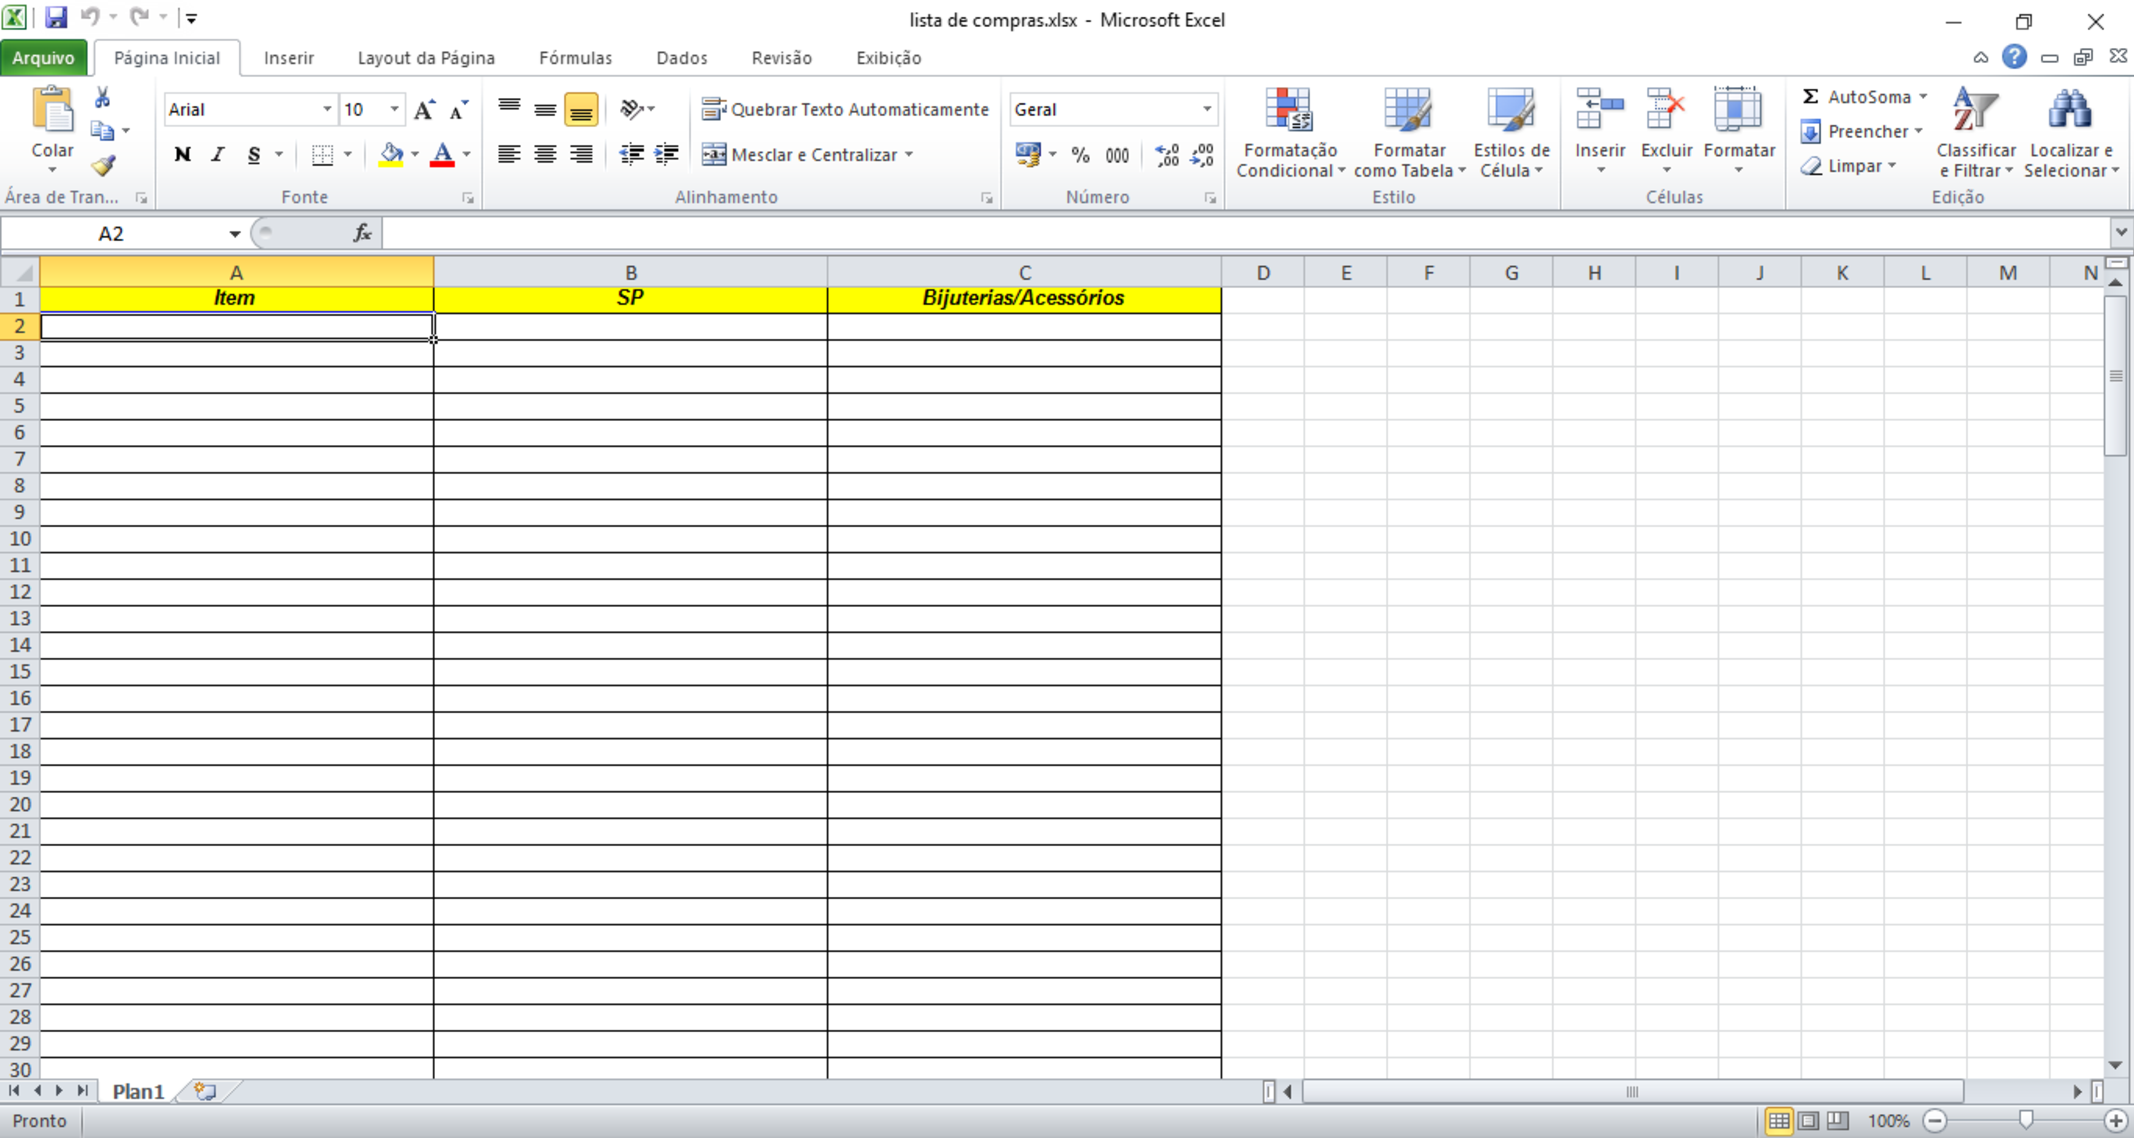
\includegraphics[width=\textwidth,keepaspectratio]{figures/lista-excel.pdf}
\caption*{\footnotesize Fonte: Produção do autor, 2016.}
\end{figure}

\begin{figure}[h]
\caption{Modelo de Impressão da Planilha}\label{fig:impressao}
\centering
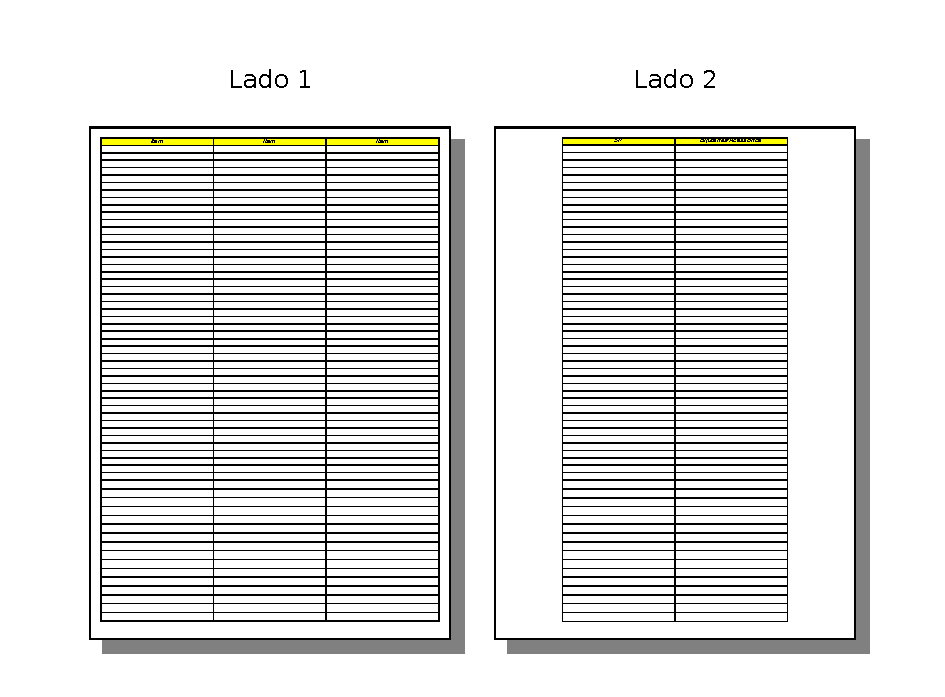
\includegraphics[width=\textwidth,keepaspectratio]{figures/modelo-impressao.pdf}
\caption*{\footnotesize Fonte: Produção do autor, 2016.}
\end{figure}


Na Figura \ref{fig:planilha} é possível visualizar a planilha descrita nesta seção. E na Figura \ref{fig:impressao} é exibida o modelo de impressão, sendo realizado em frente e verso.

\chapter{Solução Proposta}

Neste capítulo encontram-se: o levantamento, o projeto lógico e finda com o projeto do sistema.

\section{Levantamento}

Nesta seção estão expostos a visão geral do sistema e a engenharia de requisitos, para a etapa de análise do sistema eles se fazem necessários.

\subsection{Visão Geral do Sistema}

O sistema é uma aplicação para gerenciar os itens de compras, onde o usuário pode gerir listas (adicionar, editar ou remover itens), além de ser possível por usuários atribuídos marcar itens como comprados ou encerrar as listas. O acesso deverá ter algum processo de autenticação de usuário.

\subsubsection{Descrição dos usuários}

Na utilização do sistema podem ser descritos os seguintes usuários envolvidos:
\begin{itemize}
\item Funcionário: usuário que mantêm as listas, adicionando, editando e removendo itens;
\item Comprador: nível de acesso funcionário que pode realizar atividades além, que incluem marcar ou desmarcar itens como comprados e encerrar listas.
\end{itemize}

\subsection{Premissas e Restrições}

A construção dos requisitos do sistema terá a premissa e restrição listada abaixo:
\begin{itemize}
\item Premissa 1: Terá como base do sistema a planilha atualmente utilizada, cedida pela empresa;
\item Restrição 1: Acesso deve ser permitido somente por usuários cadastrados.
\end{itemize}

\subsection{Engenharia de Requisitos}

Como explicado por \citeonline{sommerville2011}, neste processo são acordados e especificados os detalhes que satisfazem os envolvidos. Há dois níveis de detalhamento dessa especificação, um para clientes e usuários outro aos desenvolvedores, alto nível e abrangente respectivamente.

Requisitos Funcionais

\subsubsection{Requisitos Funcionais}

Estes descrevem o que o sistema deve fazer, normalmente são descritos de modo abstrato para a fácil compreensão por seus usuários \cite{sommerville2011}. Puderam para o \textit{software} Buyer ser levantados os requisitos funcionais que seguem:
\begin{enumerate}
\item $[$RF001$]$ Realizar a adição de itens;
\item $[$RF002$]$ Manter as listas de itens;
\item $[$RF003$]$ Alternar o \textit{status} de compra dos itens;
\item $[$RF004$]$ Realizar encerramento das listas (manter itens não comprados);
\item $[$RF005$]$ Realizar autenticação para permitir o acesso.
\end{enumerate}

\subsubsection{Requisitos Não funcionais}


Segundo \citeonline{sommerville2011} são requisitos relacionados não diretamente as funcionalidades oferecidas aos usuários pelo sistema. Descrevem esse requisitos como: confiabilidade, desempenho, proteção ou disponibilidade.
Foram definidos para o \textit{software} Buyer os requisitos não funcionar à seguir:
\begin{enumerate}
\item $[$RNF001$]$ Acessível por navegadores, inclusive \textit{mobile};
\item $[$RNF002$]$ Interface intuitiva e minimalista;
\item $[$RNF003$]$ Tratamento em uso desconectado.
\end{enumerate}

\section{Projeto Lógico}

Nesta seção tem-se a elaboração de documentos do projeto, fase importante para melhor entendimento do sistema em desenvolvimento. Inclui-se nas seguintes subseções os diagramas UML e a modelagem da base de dados.

\subsection{Diagramas UML}

Foram desenvolvidos os diagramas de casos de uso e de classes.

\subsubsection{Diagrama de Casos de Uso}

De modo simplificado e com clareza a Figura \ref{fig:usecase} apresenta as atividade do \textit{software} Buyer.

\begin{figure}[h]
\caption{Diagrama de Casos de Uso}\label{fig:usecase}
\centering
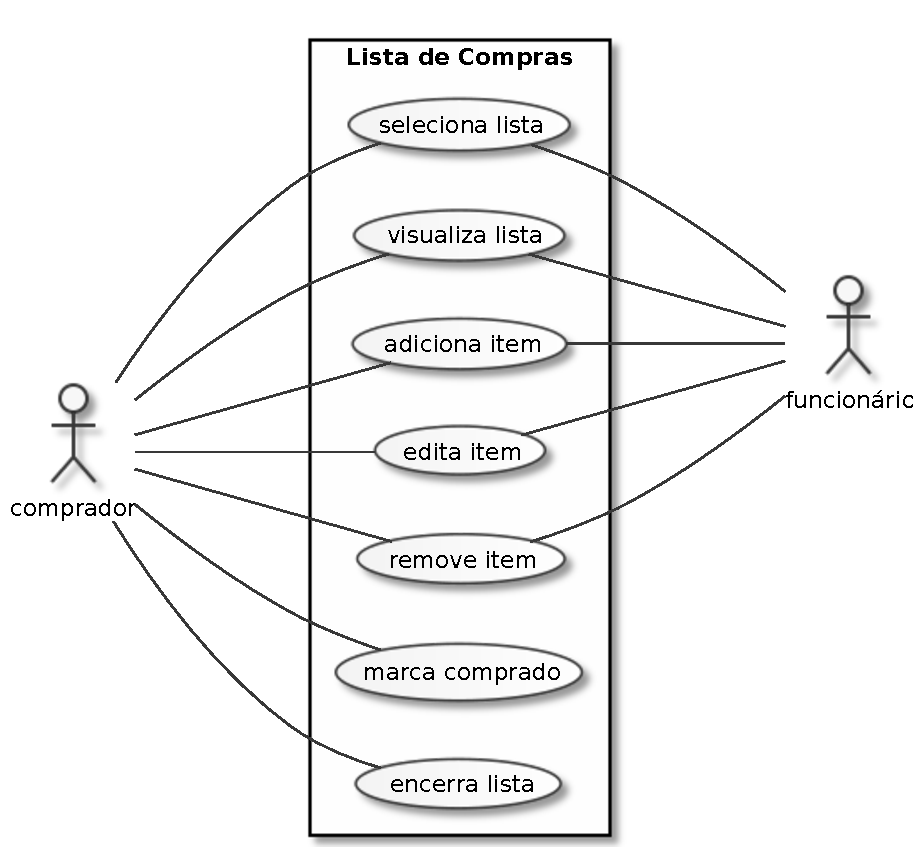
\includegraphics{figures/usecase.pdf}
\caption*{\footnotesize Fonte: Produção do autor, 2016.}
\end{figure}

\subsubsection{Diagrama de Classes}


A Figura \ref{fig:classes} ilustra o diagrama de classes do \textit{software} Buyer.

\begin{figure}[h]
\caption{Diagrama de Classes}\label{fig:classes}
\centering
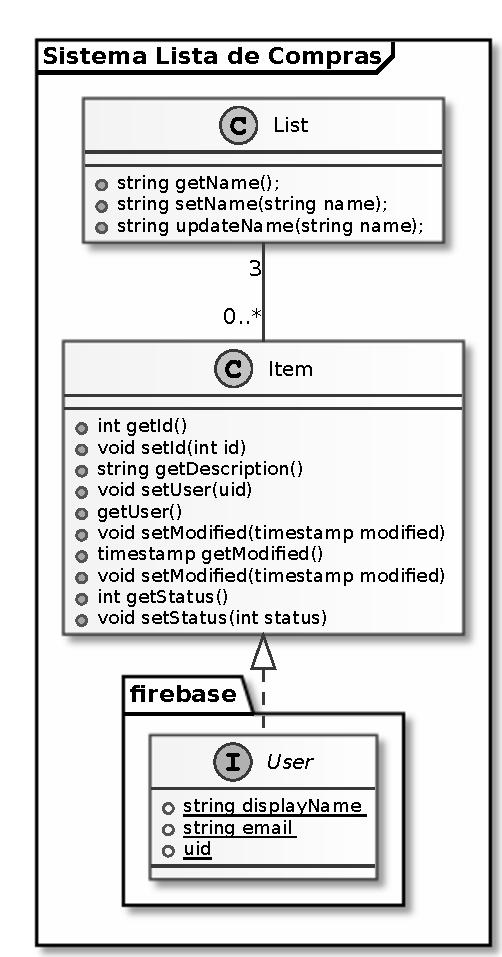
\includegraphics{figures/classes.pdf}
\caption*{\footnotesize Fonte: Produção do autor, 2016.}
\end{figure}

\postextual

\bibliographystyle{abntex2-alf}
\bibliography{references}

\end{document}
